%%% SipCon64 -- IEEE journal manuscript
%%%
%%% Style: IEEE two-column journal format (IEEEtran v1.8b, 10 pt), per the
%%% author guidelines at http://www.ieeeauthorcenter.ieee.org.
%%% Hard limit: 14 pages including author photographs and biographies, which
%%% are added at revision time -- see the reserved block before \end{document}.
%%%
%%% Build:  pdflatex main && pdflatex main
%%% IEEEtran.cls is vendored alongside this file, so no TeX Live installation
%%% of the IEEE package is required.

\documentclass[journal,10pt]{IEEEtran}

\usepackage{amsmath}
\usepackage{amssymb}
\usepackage{graphicx}
\usepackage{url}

%%% ------------------------------------------------------------------
%%% Lightweight pseudocode environment.
%%% The algorithm/algorithmic/algorithmicx packages are NOT present in this
%%% TeX installation (checked with kpsewhich), and IEEEtran.cls is vendored
%%% beside this file rather than installed, so the manuscript stays
%%% self-contained instead of taking a dependency that will not build here.
%%% Usage:
%%%   \begin{algo}{Caption text}\label{alg:foo}
%%%   line one
%%%   \Ind indented line
%%%   \end{algo}
%%% One source line = one printed line (\obeylines).
%%% ------------------------------------------------------------------
\newcounter{alg}
\newcounter{algln}
\newlength{\algnumw}\setlength{\algnumw}{1.6em}   % line-number gutter
\newlength{\alggap}\setlength{\alggap}{0.45em}    % gutter -> text gap
\newlength{\algind}\setlength{\algind}{1.0em}     % one indent level
%%% Wrapped in a minipage so the block is an unbreakable box: an algorithm
%%% that does not fit in the remaining column moves to the next column whole,
%%% instead of splitting and leaving a headerless remainder behind.
\newenvironment{algo}[1]{%
  \par\addvspace{6pt}\refstepcounter{alg}\setcounter{algln}{0}%
  \noindent\begin{minipage}{\columnwidth}%
  \hrule height0.9pt\relax
  \vspace{1.5pt}%
  \noindent\textbf{Algorithm~\thealg}\quad #1\par
  \vspace{1pt}%
  \hrule height0.4pt\relax
  \vspace{1.5pt}%
  \small\parindent=0pt\parskip=0pt\obeylines
}{%
  \par\vspace{1.5pt}%
  \hrule height0.9pt\relax
  \end{minipage}%
  \par\addvspace{6pt}%
}
%%% \aln[n] starts a numbered line indented n levels; wrapped text hangs to
%%% the text column. \aunn[n] is the same but unnumbered.
\newcommand{\aln}[1][0]{%
  \hangindent=\dimexpr\algnumw+\alggap+#1\algind\relax \hangafter=1
  \stepcounter{algln}%
  \makebox[\algnumw][r]{\footnotesize\thealgln:}\hspace{\alggap}%
  \hspace*{#1\algind}\ignorespaces}
\newcommand{\aunn}[1][0]{%
  \hangindent=\dimexpr\algnumw+\alggap+#1\algind\relax \hangafter=1
  \makebox[\algnumw][r]{}\hspace{\alggap}\hspace*{#1\algind}\ignorespaces}
%%% Require/Ensure sit flush left -- no number gutter -- with wrapped text
%%% hanging to the text column, as in the algorithmic package.
\newcommand{\areq}[1]{\hangindent=\dimexpr\algnumw+\alggap\relax\hangafter=1\textbf{Require:} #1\ignorespaces}
\newcommand{\aens}[1]{\hangindent=\dimexpr\algnumw+\alggap\relax\hangafter=1\textbf{Ensure:} #1\ignorespaces}
%%% Phase headings sit flush left, starting in the number margin, and
%%% label the numbered lines that follow them.
\newcommand{\aphase}[1]{\hangindent=\dimexpr\algnumw+\alggap\relax\hangafter=1\textit{#1}:}
\newcommand{\kw}[1]{\textbf{#1}}
\newcommand{\cmt}[1]{{\itshape\,$\triangleright$ #1}}

\begin{document}

\title{Substituting an ARX Round Function into the\\ Ascon Mode: A Hardware and Software\\ Cost Characterisation}

\author{Kaushal~Shinde% <-- replace with the full author list before submission
\thanks{Manuscript received \today.}%
\thanks{The author is with the Department, Institution, City, Country
(e-mail: azmuth6900@gmail.com).}}

\markboth{IEEE Transactions on Computer-Aided Design of Integrated Circuits and Systems}%
{Shinde: Substituting an ARX Round Function into the Ascon Mode}

\maketitle

% \begin{abstract}
% Ascon, standardised by NIST as SP 800-232, is the fastest of the eleven
% authenticated-encryption cores evaluated in this work on an FPGA target, yet
% its official reference C is the largest binary among them. The asymmetry
% follows from its bitsliced substitution round, which is shallow combinational
% logic in silicon but must be emulated with word-wide Boolean operations on a
% CPU. Ascon's specification separates its duplex-sponge mode from the
% permutation the mode invokes, which raises the question of what the mode costs
% when that round function is exchanged for an Add--Rotate--XOR one. We define
% SipCon64, which retains Ascon's mode, round constants, key-injection
% positions, padding rule and IV encoding over a 256-bit state of four 64-bit
% words, and substitutes SipHash's SIPROUND for the S-box-and-linear-layer round.
% We give a C reference and a round-per-cycle Verilog core, and evaluate eleven
% designs---Ascon-AEAD128, the proposed hybrid, and the nine remaining NIST
% Lightweight Cryptography finalists---under one reproducible flow on a Xilinx
% Artix-7 FPGA and on the SkyWater sky130 130\,nm process, together with native
% profiling of every design's reference C. The hybrid is smaller on both hardware
% targets, 874 against 1122 slice LUTs and 48\,304 against
% 62\,955\,$\mu$m$^{2}$, and is the fastest of the eleven in software at
% 367.5~MB/s against 277.0~MB/s with a $3.6\times$ smaller binary. Against this,
% its ASIC clock is $0.23\times$ Ascon's, and 38 chained carry stages account for
% approximately 94\% of its standard-cell critical path. Dedicated cryptanalysis
% of the combined construction remains future work.
% \end{abstract}

% \begin{IEEEkeywords}
% Add--Rotate--XOR (ARX), application-specific integrated circuits, Ascon,
% authenticated encryption, field-programmable gate arrays, lightweight
% cryptography, SipHash, sponge construction.
% \end{IEEEkeywords}

\IEEEpeerreviewmaketitle

% IEEE TCAD -- Introduction section
% Included by main.tex; do not compile standalone.
%
% NOTE: the citation keys below are bound to entries in refs.bib; the fields of
% those entries still need checking against the publisher record. Every numeric
% result quoted here is from this work's own measurements (see graphs/results.csv,
% software/results.csv); no figure is taken from another paper without attribution.

\section{Introduction}

\IEEEPARstart{W}{e} are surrounded by a tremendous number of lightweight
Internet of Things (IoT) devices in our day-to-day lives, includ-
ing smartwatches, home automation systems, and industrial
sensors . These devices operate across four architectural
layers: the application layer (mobile apps, voice recognition),
the data processing layer (CPU/GPU compute), the network
layer (Wi-Fi, Bluetooth), and the sensing layer (thermostats,
transducers) . Every day, these devices communicate over
local networks and the broader Internet, capturing and trans-
mitting sensitive personal and environmental data – creating a
broad attack surface that spans physical attacks, side-channel
exploitation, cryptanalysis, and network eavesdropping .

\subsection{AES and Its Limits}

 for lightweight Internet of Things (IoT) devices like medical implants, smart meters, and environmental sensors, AES is computationally infeasible due to severe hardware and power constraints. AES relies on a large 128-bit block size and complex matrix transformations that demand significant RAM, ROM, and processing cycles. This forces basic microcontrollers to stay awake longer, rapidly draining their small batteries, and requires too many hardware logic gates on tiny microchips. To connect these devices securely, engineers previously used alternative ciphers like PRESENT, Trivium, or SIMON and SPECK, which relied on ultra-simple logical operations to minimize chip space and power consumption. However, this efficiency came with dangerous trade-offs: these older ciphers often used small 64-bit blocks that leak information when transmitting large amounts of IoT data, offered weaker security margins, and lacked native authentication, meaning they could not stop hackers from tampering with commands or sending fake data. Ascon solves this IoT security crisis by using a highly efficient "sponge" design. It delivers ironclad, modern 128-bit security alongside native Authenticated Encryption with Associated Data (AEAD) in a single step. This allows battery-powered IoT devices to encrypt and verify their data simultaneously, consuming minimal power and chip space without sacrificing security.




\subsection{Origin of  Ascon}

Securing resource-constrained Internet of Things hardware presents a difficult balance between cryptographic security and physical resource limits. Early deployment strategies relied on dedicated lightweight block ciphers like PRESENT, SIMON, and SPECK, or stream ciphers such as Trivium and Grain-128AEAD. While these early primitives achieved low gate counts in hardware, their architectural reliance on small 64-bit blocks created significant security trade-offs. Processing long data streams under a single key exposed these systems to birthday-bound state-leakage attacks. Furthermore, because these early ciphers lacked integrated Authenticated Encryption with Associated Data features, designers had to pair encryption engines with external Message Authentication Code blocks. Combining separate algorithms added substantial memory and hardware overhead, negating much of the original resource savings. Engineered in 2014 by researchers from Graz University of Technology, Infineon Technologies, and Lamarr Security Research, Ascon was designed to overcome these structural limits as a unified cryptographic suite built on a flexible 320-bit sponge permutation core. This shared mathematical state natively supports both AEAD and secure cryptographic hashing within the exact same structural pipeline, significantly reducing code size and silicon area while maintaining strong mathematical security margins across constrained microcontrollers and dedicated integrated circuits.

Ascon’s transition from a research proposal to a global standard was driven by success in two key international selection competitions. The CAESAR competition evaluated 57 initial algorithms over multiple elimination rounds, ultimately selecting Ascon in 2019 as the Primary Choice for Use Case 1, which designated lightweight applications. While bit-oriented stream ciphers like ACORN offered lower gate counts in specialized hardware, ACORN suffered from high software overhead and significant side-channel vulnerabilities, leading the committee to favor Ascon's versatile hardware-software balance. Ascon subsequently entered NIST’s Lightweight Cryptography selection process among 56 competing candidates. Following multi-year evaluations focused on hardware gate efficiency, software speed, memory bounds, and physical attack resilience, NIST narrowed the pool to ten finalists in 2021 before officially declaring Ascon the winning primary standard for global lightweight cryptography in February 2023.

Ascon outperformed the remaining nine NIST LWC finalists because it avoided the specific architectural weaknesses that limited competing designs. Hardware-centric primitives such as TinyJambu and Grain-128AEAD achieved small gate footprints on application-specific integrated circuits through bitwise silicon operations, but this design caused severe processing bottlenecks on standard microcontrollers. In contrast, Ascon uses 64-bit word operations that map directly to standard register architectures without sacrificing hardware efficiency. Similarly, side-channel vulnerable ciphers like Romulus, GIFT-COFB, and PHOTON-Beetle required heavy masking countermeasures to protect against physical power-analysis attacks, which drastically inflated their memory usage and execution latency. Ascon mitigates this issue by employing a low-degree, degree-2, 5-bit substitution box that enables efficient, low-overhead hardware masking. Finally, large-state ciphers like Xoodyak and Sparkle achieved high software speeds but demanded excessive RAM and ROM allocation, rendering them impractical for the most memory-restricted microchips. By balancing software throughput, hardware area, masking simplicity, and state size inside a single unified sponge construction, Ascon provided chip designers with maximum functional utility per unit of silicon area.


\subsection{Where Ascon Is Costly}

Ascon is highly optimized for hardware. Because its core operations use simple bitwise logic rather than complex memory lookups, it can process data in parallel with almost zero delay. In our tests on a Xilinx Artix-7 FPGA, Ascon was the fastest of all eleven designs, reaching 241.4 MHz.

However, this hardware efficiency creates challenges for software. A standard CPU has to manually emulate these parallel hardware operations, which requires extra instructions. To keep the software running fast, the official C code expands these instructions significantly. As a result, Ascon requires 15,569 bytes of ROM—the largest memory footprint of all tested designs, and 3.6 times larger than its smallest competitor. For constrained devices where flash memory is strictly limited, this creates a significant trade-off: Ascon delivers top-tier hardware speed, but demands massive software storage.

\subsection{ARX Primitives}

In contrast to hardware-focused designs, Add-Rotate-XOR (ARX) algorithms are optimized for software efficiency. Because they rely entirely on modular addition, bitwise rotation, and XOR, they work more optimally  to standard CPU instructions without requiring memory lookup tables. Furthermore, their execution time does not depend on the data being processed. This makes them naturally immune to cache-timing attacks.And this is the exact issue that bitslicing attempts to solve. Well-known existing algorithms like ChaCha20, BLAKE2, and SipHash use this ARX structure, which is why ChaCha20 is widely deployed on systems lacking dedicated AES hardware.

SipHash is one of the most efficient example of this design. Its core function, SIPROUND, processes a 256-bit state using only four additions, six rotations, and four XOR operations. It was specifically engineered to process short data inputs rapidly on processors with limited resources.

\subsection{Motivation Behind Substituting the Round Function}

Ascon clearly separates its outer operating mode from its inner mixing engine, meaning the outer structure works perfectly fine regardless of how the inside is built. This allows us to experiment with keeping Ascon's proven mode while replacing its current inner engine with an ARX design. We are making this swap because the two approaches have opposite strengths: Ascon's current setup is highly efficient for physical hardware but clunky and slow in software, whereas ARX uses basic math that runs incredibly fast in software but is difficult to build into chips. By combining Ascon's mode with an ARX engine, we aim to trade hardware efficiency for better software speed. Because this specific hybrid has never been tested across both software and hardware, we need to find out if it combines the best features of both or just inherits their worst flaws.


\subsection{Contributions}

This paper introduces a kind of hybrid design of ascon aead and siphash and measures its performance. We call it Ascon-SipHash-r64. It keeps Ascon's overall outer structure—such as its operating mode, keys, and padding—but replaces Ascon's round function in full, both the substitution layer and the linear diffusion layer, with SipHash's SIPROUND, retaining Ascon's round-constant addition ahead of it. The total data size is shrunk to 256 bits, split into four 64-bit chunks. By keeping the processing block at 64 bits, we maintain the same 192-bit security reserve as standard Ascon-AEAD128. This new setup uses 10 rounds ($p^{10}$) to start and finish, and 6 rounds ($p^{6}$) for each block of data.

Our main contributions are:

\begin{itemize}
\item \emph{A complete design:}We have developed a new version of ascon aead and implemented in both c and verilog.

\item \emph{A fair, head-to-head performance test:} We compared 11 different cryptography engines, including standard Ascon, our new mixed design, and nine other NIST finalists. We tested all of them using the exact same methods on an FPGA and a standard chip-making process (130nm). We also measured their software speeds. All of our testing tools are being released publicly with this paper.
\item \emph{A clear measurement of the pros and cons:} The mixed version takes up less physical space on chips than standard Ascon (874 vs. 1122 Slice LUTs, and 48,304 vs. 62,955 µm²). It is also the fastest of all 11 designs in software, hitting 367.5 MB/s compared to Ascon's 277.0 MB/s, while taking up about 3.6 times less memory. However, its hardware clock speed drops heavily to just 23\% of standard Ascon's speed. We proved that this huge slowdown is caused by a long chain of basic math steps that create a bottleneck in the chip's processing path.
\end{itemize}

The remainder of this paper is organised as follows. Section~\ref{sec:related}
places the substitution against prior work on sponge modes, ARX primitives and
the benchmarking of the NIST LWC candidates. Section~\ref{sec:prelim}
reviews the Ascon mode and SIPROUND. Section~\ref{sec:construction} specifies
the hybrid. Section~\ref{sec:impl} describes the hardware and software
implementations and the evaluation flow. Section~\ref{sec:results} presents the
measured comparison across all eleven designs. Section~\ref{sec:discussion}
analyses the critical path.
Section~\ref{sec:conclusion} concludes.


% IEEE TCAD -- Related Work section
% Included by main.tex; do not compile standalone.
%
% NOTE: as in introduction.tex, the citation keys below are bound to entries in
% refs.bib whose volume/page/date fields still need checking against the
% publisher record. No numeric claim about another author's work is quoted
% here; comparisons to prior measurements are deliberately qualitative, because
% this paper's own flow (Section~\ref{sec:impl}) is not the flow those papers
% used and the absolute values are not comparable.

\section{Related Work}
\label{sec:related}

Our experiment connects four main areas of prior research: permutation-based modes that separate the outer framework from the inner engine, making this kind of round substitution possible; ARX-based designs that provide our replacement round along with their well-known hardware and software trade-offs; existing benchmark studies of the NIST Lightweight Cryptography (LWC) candidates, which our eleven-design evaluation expands upon rather than repeats; and the published implementation literature on Ascon itself.

\subsection{Permutation-Based Modes and the Mode/Primitive Split}
The sponge construction \cite{sponge} and its duplex variant \cite{duplex} are built in two parts: the outer structure (the mode) and the inner mixing engine (the $b$-bit permutation). The mode governs how data is absorbed into the rate ($r$), while the capacity ($c$) is never touched by data directly---the property on which its security rests---and assumes the inner permutation is indistinguishable from a random one. Jovanovic \emph{et al.} \cite{jlm} proved that sponge-based authenticated encryption can achieve security beyond the birthday bound in the capacity, which forms the mathematical basis for Ascon's security claims \cite{caesar}.

Because the mode treats the permutation as a black box, the permutation can be exchanged without breaking the mode's mechanics. 
so Our design replaces Ascon's round function in full---both the 5-bit substitution layer and the linear diffusion layer---with SIPROUND from SIPHASH \cite{siphash}, retains Ascon's round-constant addition ahead of it, and narrows the state from five 64-bit words to four. The two layers are replaced together rather than separately because a single SIPROUND supplies, through its Addition--Rotation--XOR (ARX) operations, both the non-linearity and the inter-word mixing that Ascon divides between them.

Mixing modes and permutations is standard practice. Xoodyak \cite{xoodyak} runs its Cyclist mode over the Xoodoo permutation, while ISAP \cite{isap}, itself one of the nine finalists measured here, uses Ascon's permutation inside a different, leakage-resilient mode. However, this paper does the reverse: we hold a standardized mode completely fixed, swap its round function for one from a different design family, and measure the resulting costs across hardware and software targets.

\subsection{ARX Primitives and Their Cost Asymmetry}
Add-Rotate-XOR (ARX) designs, such as Salsa20 and ChaCha \cite{salsa,chacha}, BLAKE2 \cite{blake2}, SPECK \cite{simonspeck}, and SipHash \cite{siphash}, rely entirely on modular addition for nonlinearity. Because modern CPUs natively handle these operations without using lookup tables, ARX ciphers are extremely fast, compact, and naturally immune to the cache-timing side-channel attacks demonstrated by Bernstein against AES \cite{aes-cache}.

However, ARX designs struggle in hardware. Modular addition requires a carry propagation, which creates physical delays in the circuit. The SIMON and SPECK families \cite{simonspeck} clearly illustrate this divide: SIMON was built without addition for hardware efficiency, while SPECK relies on addition for software speed. SPARKLE, the only ARX-based NIST LWC finalist \cite{sparkle}, is built on a custom ARX-box called Alzette \cite{alzette}, designed to obtain strong cryptographic properties at bounded circuit depth. SPARKLE is the natural reference point for ARX in this field, though not a like-for-like one: its permutation is wider and performs considerably more work per invocation than SIPROUND over a 256-bit state, so Section~\ref{sec:results} reports it as context rather than as a matched ARX baseline.

The specific cost this paper measures---the 64-bit modular addition setting the critical path of a SipHash-derived round in silicon---has been identified independently. HAxSH \cite{haxsh} takes SipHash's round as given and attacks exactly that bottleneck, substituting approximate adders with shortened carry propagation for the exact ones and reporting substantial latency and power reductions from ASIC synthesis, with the resulting loss of exactness assessed through statistical testing and MILP-based differential and linear analysis. That work and this one share a diagnosis and differ in response: HAxSH changes the adder and keeps the construction exact nowhere, whereas this paper leaves SIPROUND untouched and asks what an unmodified ARX round costs when carried into a standardized AEAD mode. Its results are the natural point of comparison for any attempt to reduce the critical path reported in Section~\ref{sec:discussion}.

For our experiment, we substitute Ascon's s-box and linear diffusion layer with SIPROUND from SipHash \cite{siphash}. SipHash was originally designed as a short-input pseudorandom function for hash tables rather than for bulk encryption; the grounds for carrying its round into an AEAD permutation are set out above.

\subsection{Benchmarking of the NIST LWC Candidates}
The NIST Lightweight Cryptography (LWC) process produced extensive benchmarking data. Hardware comparisons were standardized using the GMU Hardware API \cite{lwc-api}---the interface the nine finalist cores measured here implement---allowing for consistent FPGA \cite{mohajerani} and ASIC \cite{aagaard} evaluations as summarized by NIST \cite{nist-lwc-report, nist-lwc-final}. In software, candidates were benchmarked across various microcontrollers \cite{renner,weatherley}. 

Our evaluation differs from these campaigns in two ways. First, our goal is not to rank candidates; instead, we use the eleven-design field as a calibration scale to measure the precise impact of our ARX substitution. Second, our software tests use unmodified C code on a standard x86-64 processor rather than tuned embedded code.Because a standard PC compiler optimizes code very differently than an embedded compiler, you cannot compare the exact performance numbers—especially the code size—to previous embedded studies \cite{renner,weatherley};. You can only compare the *relative rankings*, meaning which algorithm placed first, second, or third.

\subsection{Ascon Implementations}
Ascon's 5-bit S-box has algebraic degree 2, which makes it unusually cheap to mask against side-channel attacks. Dedicated Ascon hardware and its side-channel behaviour were studied early by Gro\ss{} \emph{et al.} \cite{gross}, and a considerable number of cores have followed, particularly since standardization as NIST SP 800-232 \cite{nist-sp800-232}. The Ascon-AEAD128 core measured in our paper is not intended to compete with these highly optimized, protected versions. Instead, it is a basic, round-per-cycle implementation built specifically to serve as a direct, apples-to-apples control group for our hybrid design using the exact same toolchain.


In summary, this paper presents a controlled substitution rather than a new cipher design. We keep Ascon's mode fixed, replace its standard round function with SIPROUND, and measure the results in C and Verilog against ten existing algorithms using consistent hardware and software flows. The security rationale for the resulting hybrid rests on the maturity of the two components it combines; dedicated cryptanalysis of the combination itself remains future work.

%%% ------------------------------------------------------------------
%%% Remaining sections. The labels are declared here so that the forward
%%% references at the end of the Introduction resolve; replace each stub
%%% with its section file as it is written.
%%% ------------------------------------------------------------------

% IEEE TCAD -- Background and Motivation
% Included by main.tex; do not compile standalone.
%
% Structural details were read off the sources vendored in this repository,
% not quoted from the specifications:
%   Ascon-AEAD128 mode      ascon-aead128/aead.c    (ASCON_128A_IV path)
%   Ascon round function    ascon-aead128/round.h
%   SIPROUND                siphash/siphash.c
% Kept deliberately brief: Section~\ref{sec:construction} specifies the hybrid
% in full, so this section only establishes why the substitution is worth
% making. Notation: $\oplus$ exclusive-or, $\boxplus$ addition mod $2^{64}$,
% ROL/ROR rotation, all words 64 bits.

\section{Background and Motivation}
\label{sec:background}

\subsection{From AES to Lightweight AEAD}

AES \cite{fips197} is the standard against which lightweight encryption is measured, and it struggles on small devices for specific reasons. Fast software versions use memory tables, making their timing vary and leaving them open to cache-timing attacks \cite{aes-cache}. Versions without tables avoid this but are much slower. On physical chips, its S-box uses a lot of logic gates, and protecting it from power-monitoring attacks is very expensive. Also, AES only hides data; it needs extra steps and more space or time to prove the data hasn't been tampered with.

Lightweight options that came before the NIST Lightweight Cryptography process solved some problems but created others. Ciphers like PRESENT, SIMON, and SPECK \cite{simonspeck} take up very little space, but most use 64-bit blocks, which limits how much data they can safely process. None of them provide built-in authentication.

\subsection{Ascon}

Ascon \cite{caesar,nist-sp800-232} fixes both problems at once. It uses a 320-bit core process (a permutation) inside a sponge design. The data enters and leaves through a ``rate'' section, while a ``capacity'' section remains untouched to keep the system secure \cite{sponge,duplex}. It encrypts and authenticates data at the exact same time, so it doesn't need extra pieces, and it can also hash data. Ascon won the CAESAR lightweight competition and was chosen as the NIST standard in 2023 \cite{nist-lwc-final}, becoming SP 800-232 \cite{nist-sp800-232}.

Inside Ascon, one round adds a constant, applies a 5-bit S-box, and then mixes the data. The S-box uses a method called \emph{bitslicing}, where basic math operations process 64 S-boxes at once. This makes Ascon very cheap to protect against power attacks.

This setup is perfect for physical hardware---it takes very few gates and causes no delays, measuring just three logic levels deep as shown in Section~\ref{sec:results}. However, it is terrible for software. Regular processors cannot run bitsliced math natively, so the software must use a lot of code to fake it. This results in the largest software program among all eleven designs we tested.

\subsection{Why SipHash}

SipHash \cite{siphash} has the exact opposite strengths. It is an Add--Rotate--XOR (ARX) design. Its inner engine, SIPROUND, relies entirely on basic addition, rotation, and XOR steps on a 256-bit state of four words $(v_0,v_1,v_2,v_3)$,
\begin{equation}
\begin{array}{ll}
v_0 \mathrel{+}= v_1 & v_2 \mathrel{+}= v_3\\
v_1 \mathrel{\lll}= 13 \qquad & v_3 \mathrel{\lll}= 16\\
v_1 \mathrel{\oplus}= v_0 & v_3 \mathrel{\oplus}= v_2\\
v_0 \mathrel{\lll}= 32 & \\[2pt]
v_2 \mathrel{+}= v_1 & v_0 \mathrel{+}= v_3\\
v_1 \mathrel{\lll}= 17 & v_3 \mathrel{\lll}= 21\\
v_1 \mathrel{\oplus}= v_2 & v_3 \mathrel{\oplus}= v_0\\
v_2 \mathrel{\lll}= 32 &
\end{array}
\label{eq:sipround}
\end{equation}

This adds up to four additions, six rotations, and four XORs. Three things make this great for our experiment. First, a standard 64-bit processor can run every step in a single, fast instruction without needing lookup tables. This makes it compact, fast, and safe from timing attacks in software, much like ChaCha20 \cite{chacha}. Second, it is highly trusted, with a decade of real-world use and security testing. Third, it is small, using four words instead of Ascon's five.

We write \eqref{eq:sipround} in the two-column form used by its designers \cite{siphash}, because the columns carry information: the left and right halves of each block are independent and may be evaluated at the same time. Note that the two columns exchange partners between the upper and lower blocks---$v_0$ pairs with $v_1$ and then with $v_3$---which is the crossing visible in a datapath drawing of the round.

That structure is what fixes its hardware cost. Every addition forces the chip to carry numbers down a 64-bit chain, and \eqref{eq:sipround} contains four of them, but they are not linked end to end: the upper two take independent inputs, and the lower two each wait on both upper results while remaining independent of one another. One round therefore costs \emph{two} chained additions, not four. Two is still enough to dominate the delay, because no rearrangement of the surrounding rotations and XORs shortens a carry chain.

\subsection{Motivation}
\label{sec:motivation}

The S-box is the only reason Ascon is bulky in software. The rest of its math maps perfectly to normal software instructions. In hardware, that same S-box costs almost nothing. The software problem is tied to one specific part for a specific reason.

Because Ascon's outer structure (the mode) is completely separate from its inner engine, we can swap the engine while keeping the keys, padding, and security setup exactly the same. This allows for a direct experiment: replace the part that causes software bloat with an engine built from basic CPU instructions, keep everything else the same, and measure the results. Since SIPROUND mixes data well on its own, it replaces both Ascon's S-box and its mixing layer.


\section{Architecture of SipCon64}
\label{sec:architecture}

\subsection{The Proposed Construction}

We introduce \emph{SipCon64}, a new encryption design. It keeps Ascon-AEAD128's outer sponge structure intact but completely replaces its inner mixing engine. We remove Ascon's S-box and linear layers entirely, swapping them out for SipHash's SIPROUND engine. However, we keep Ascon's method for adding round constants. Everything else remains exactly the same: how data enters (rate and capacity), the padding rules, the separation flags, where the key is added, and the starting setup.

Ascon's inner math is great for physical chips but forces software to use clunky workarounds. SIPROUND uses basic math that software runs instantly, but it forces physical chips to wait on slow addition steps. By swapping the engine while keeping the outer shell the same, we can isolate the exact cost of the engine on different devices. We report these measurements in Section~\ref{sec:results}.

\subsection{Components}

\subsubsection{State}
Following Ascon's design \cite{caesar}, the internal memory (the state) is written as:
\begin{equation}
S = S_r \,\|\, S_c = x_0 \,\|\, x_1 \,\|\, x_2 \,\|\, x_3,
\label{eq:state}
\end{equation}
which is four 64-bit words totaling 256 bits. We use $\lfloor X\rfloor_{\ell}$ to mean the last bits of $X$, and $\lceil X\rceil_{\ell}$ for the first bits. We treat the state as a sequence of bytes starting at the lowest byte of $x_0$.

\subsubsection{Rate and capacity}
The state is split into an outer part ($S_r = x_0$) with $r=64$ bits, and an inner part ($S_c = x_1\Vert{}x_2\Vert{}x_3$) with $c=192$ bits. Because SIPROUND only processes four words, the total memory shrinks from Ascon's 320 bits down to 256. We have to take those missing 64 bits from somewhere. We decided to cut the rate (the data input size) to 64 bits so we could keep the capacity at 192 bits. Keeping a large capacity maintains Ascon-AEAD128's security strength. The trade-off is that each step processes less data.

\subsubsection{Key, nonce and tag}
Just like Ascon-AEAD128, the key, nonce (a single-use number), and tag are all 128 bits long. We write them as $K = K_0\Vert{}K_1$ and $N = N_0\Vert{}N_1$.

\subsubsection{Initial value}
The starting value (IV) uses the exact same layout as Ascon-AEAD128. We simply add the letter 'S' (\texttt{0x53}) at the top to indicate that it uses SipHash:
\begin{equation}
\mathit{IV} = \texttt{0x00530800806A0001}.
\label{eq:iv}
\end{equation}
Because the IV includes the specific round counts, a SipCon64 setup will never accidentally overlap or collide with a standard Ascon-AEAD128 setup.

\subsection{The Round Function and the Permutations}

\begin{figure*}[!t]
\centering
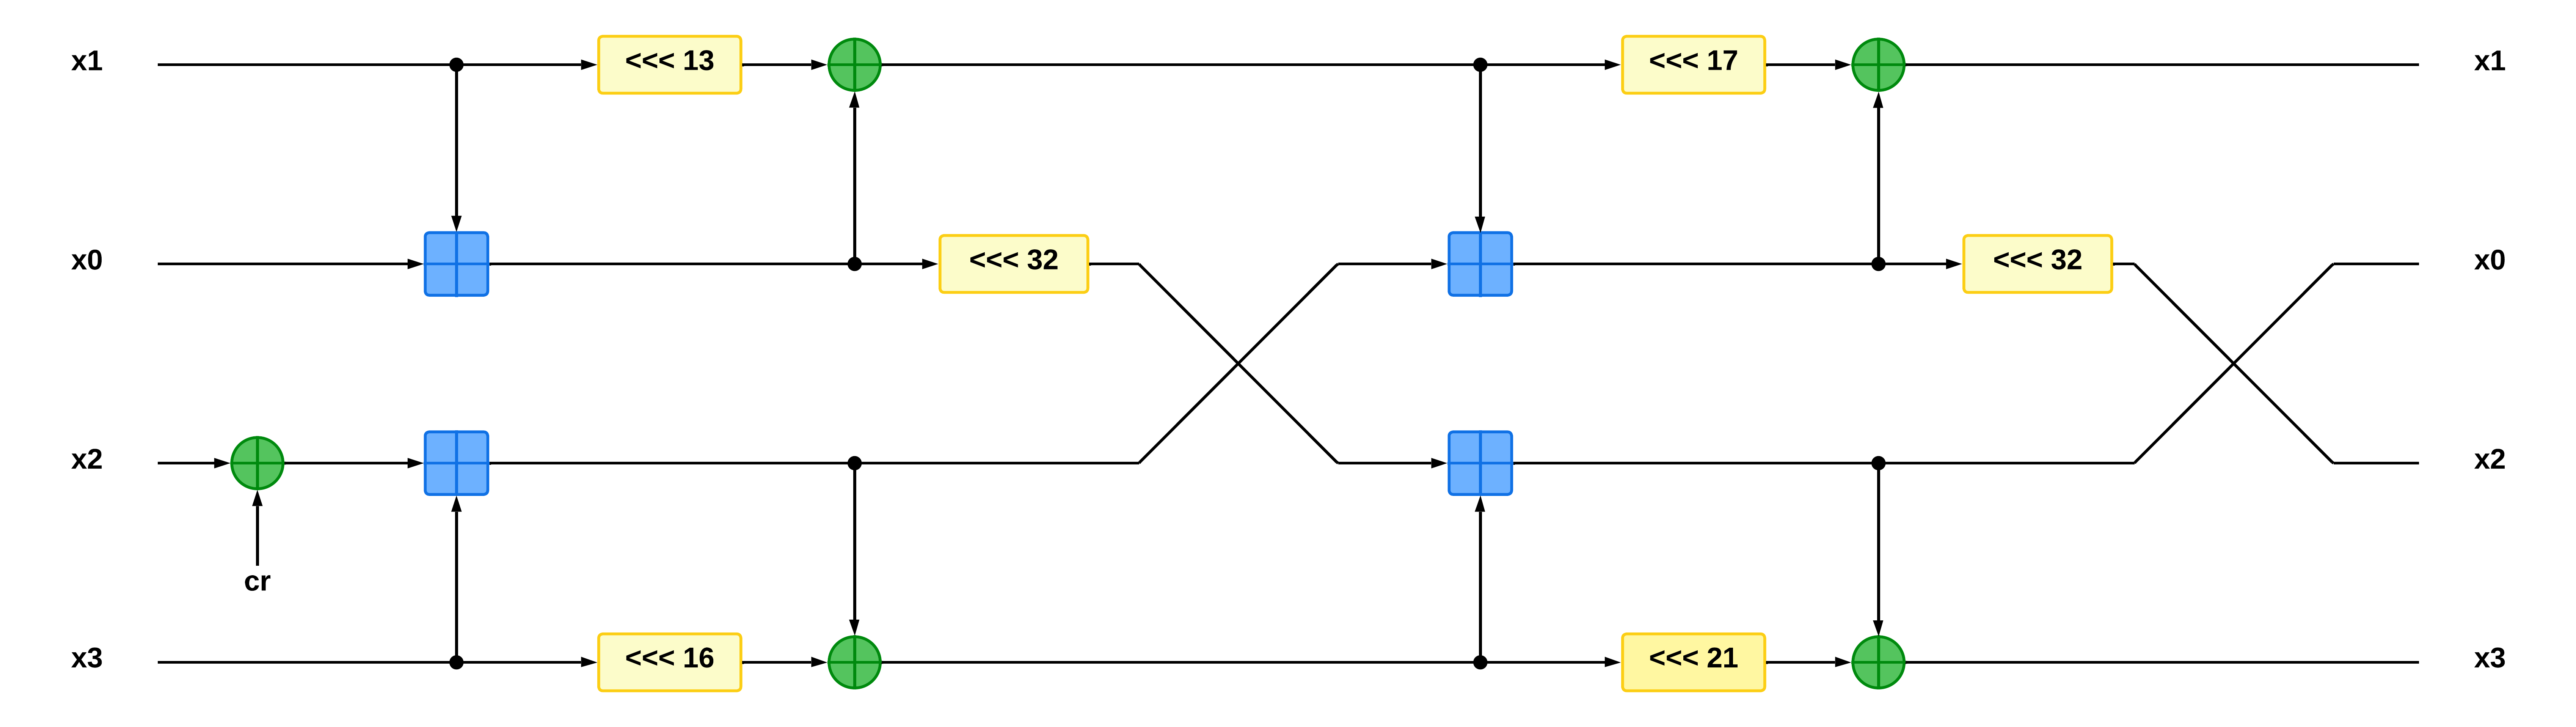
\includegraphics[width=\textwidth]{images/Round-Function}
\caption{One SipCon64 round, $p = \mathrm{SIPROUND}\circ p_C$. The round constant $c_r$ enters the capacity word $x_2$ on the left. Blue squares are additions modulo $2^{64}$, green circles are exclusive-ors, and yellow boxes are cyclic left rotations. The two additions in each half happen at the same time. The crossing in the middle happens because $x_0$ and $x_2$ switch roles in \eqref{eq:sipround}, which is swapped back on the right so the words exit in their original places.}
\label{fig:round}
\end{figure*}

\subsubsection{Symbols used in the figures}
Both diagrams use the same symbols. A plus in a square, $\boxplus$, is addition
modulo $2^{64}$; a plus in a circle, $\oplus$, is exclusive-or. A rounded box
is a cyclic left rotation by the number of positions printed inside it. A
filled dot on a wire is a fan-out, and a crossing of two wires is a relabelling
only. In Fig.~\ref{fig:mode}, a tall grey bar is a permutation call labelled
with its round count, and a slash across a wire gives that bus width in bits.

One mixing round combines two steps:
\begin{equation}
p = \mathrm{SIPROUND}\circ p_{C},
\label{eq:round}
\end{equation}
which is mapped out in Fig.~\ref{fig:round}.

\subsubsection{Constant addition}
First, $p_C$ adds a round constant to the capacity word $x_2$, just like standard Ascon \cite{caesar}:
\begin{equation}
x_2 \leftarrow x_2 \oplus c_r .
\label{eq:pc}
\end{equation}
SipCon64 uses Ascon's original twelve constants. If a phase uses fewer rounds, it takes constants from the end of the list. A 10-round mix starts at \texttt{0xd2}, and a 6-round mix starts at \texttt{0x96} (Table~\ref{tab:rc}).

\subsubsection{SIPROUND}
Next, we apply SIPROUND \cite{siphash} to the four words. We write it in two columns to show which math steps happen at the same time:
\begin{equation}
\begin{array}{ll}
x_0 \mathrel{+}= x_1 & x_2 \mathrel{+}= x_3\\
x_1 \mathrel{\lll}= 13 \qquad & x_3 \mathrel{\lll}= 16\\
x_1 \mathrel{\oplus}= x_0 & x_3 \mathrel{\oplus}= x_2\\
x_0 \mathrel{\lll}= 32 & \\[2pt]
x_2 \mathrel{+}= x_1 & x_0 \mathrel{+}= x_3\\
x_1 \mathrel{\lll}= 17 & x_3 \mathrel{\lll}= 21\\
x_1 \mathrel{\oplus}= x_2 & x_3 \mathrel{\oplus}= x_0\\
x_2 \mathrel{\lll}= 32 &
\end{array}
\label{eq:sipround}
\end{equation}
The left and right columns do not depend on each other, meaning a processor can run them simultaneously. Between the top and bottom halves, $x_0$ and $x_2$ switch partners. You can see this crossover in the middle of Fig.~\ref{fig:round}.

This layout is very important for hardware. Even though the round uses four addition steps, they do not happen one after another. The two top additions process at the same time, and the two bottom additions process at the same time. Therefore, the chip only suffers the delay of \emph{two} stacked additions per round, not four.

\subsubsection{The two permutations}
We use two different mixing strengths. We use 10 rounds ($p^{10}$) at the very beginning and end to maximize security where attackers have the most control. We use a faster 6-round mix ($p^{6}$) in the middle between data blocks.

\begin{table}[!t]
\centering
\caption{Round constants $c_r$, kept exactly as they are in Ascon. A shorter mix uses the constants at the end of the list, so $p^{10}$ starts at \texttt{0xd2} and $p^{6}$ starts at \texttt{0x96}.}
\label{tab:rc}
\small
\begin{tabular}{ccl@{\qquad}ccl}
\hline
$p^{10}$ & $p^{6}$ & $c_r$ & $p^{10}$ & $p^{6}$ & $c_r$\\
\hline
0 & & \texttt{0xd2} & 5 & 1 & \texttt{0x87}\\
1 & & \texttt{0xc3} & 6 & 2 & \texttt{0x78}\\
2 & & \texttt{0xb4} & 7 & 3 & \texttt{0x69}\\
3 & & \texttt{0xa5} & 8 & 4 & \texttt{0x5a}\\
4 & 0 & \texttt{0x96} & 9 & 5 & \texttt{0x4b}\\
\hline
\end{tabular}
\end{table}

\subsection{The Duplex Mode}

\begin{figure*}[!t]
\centering
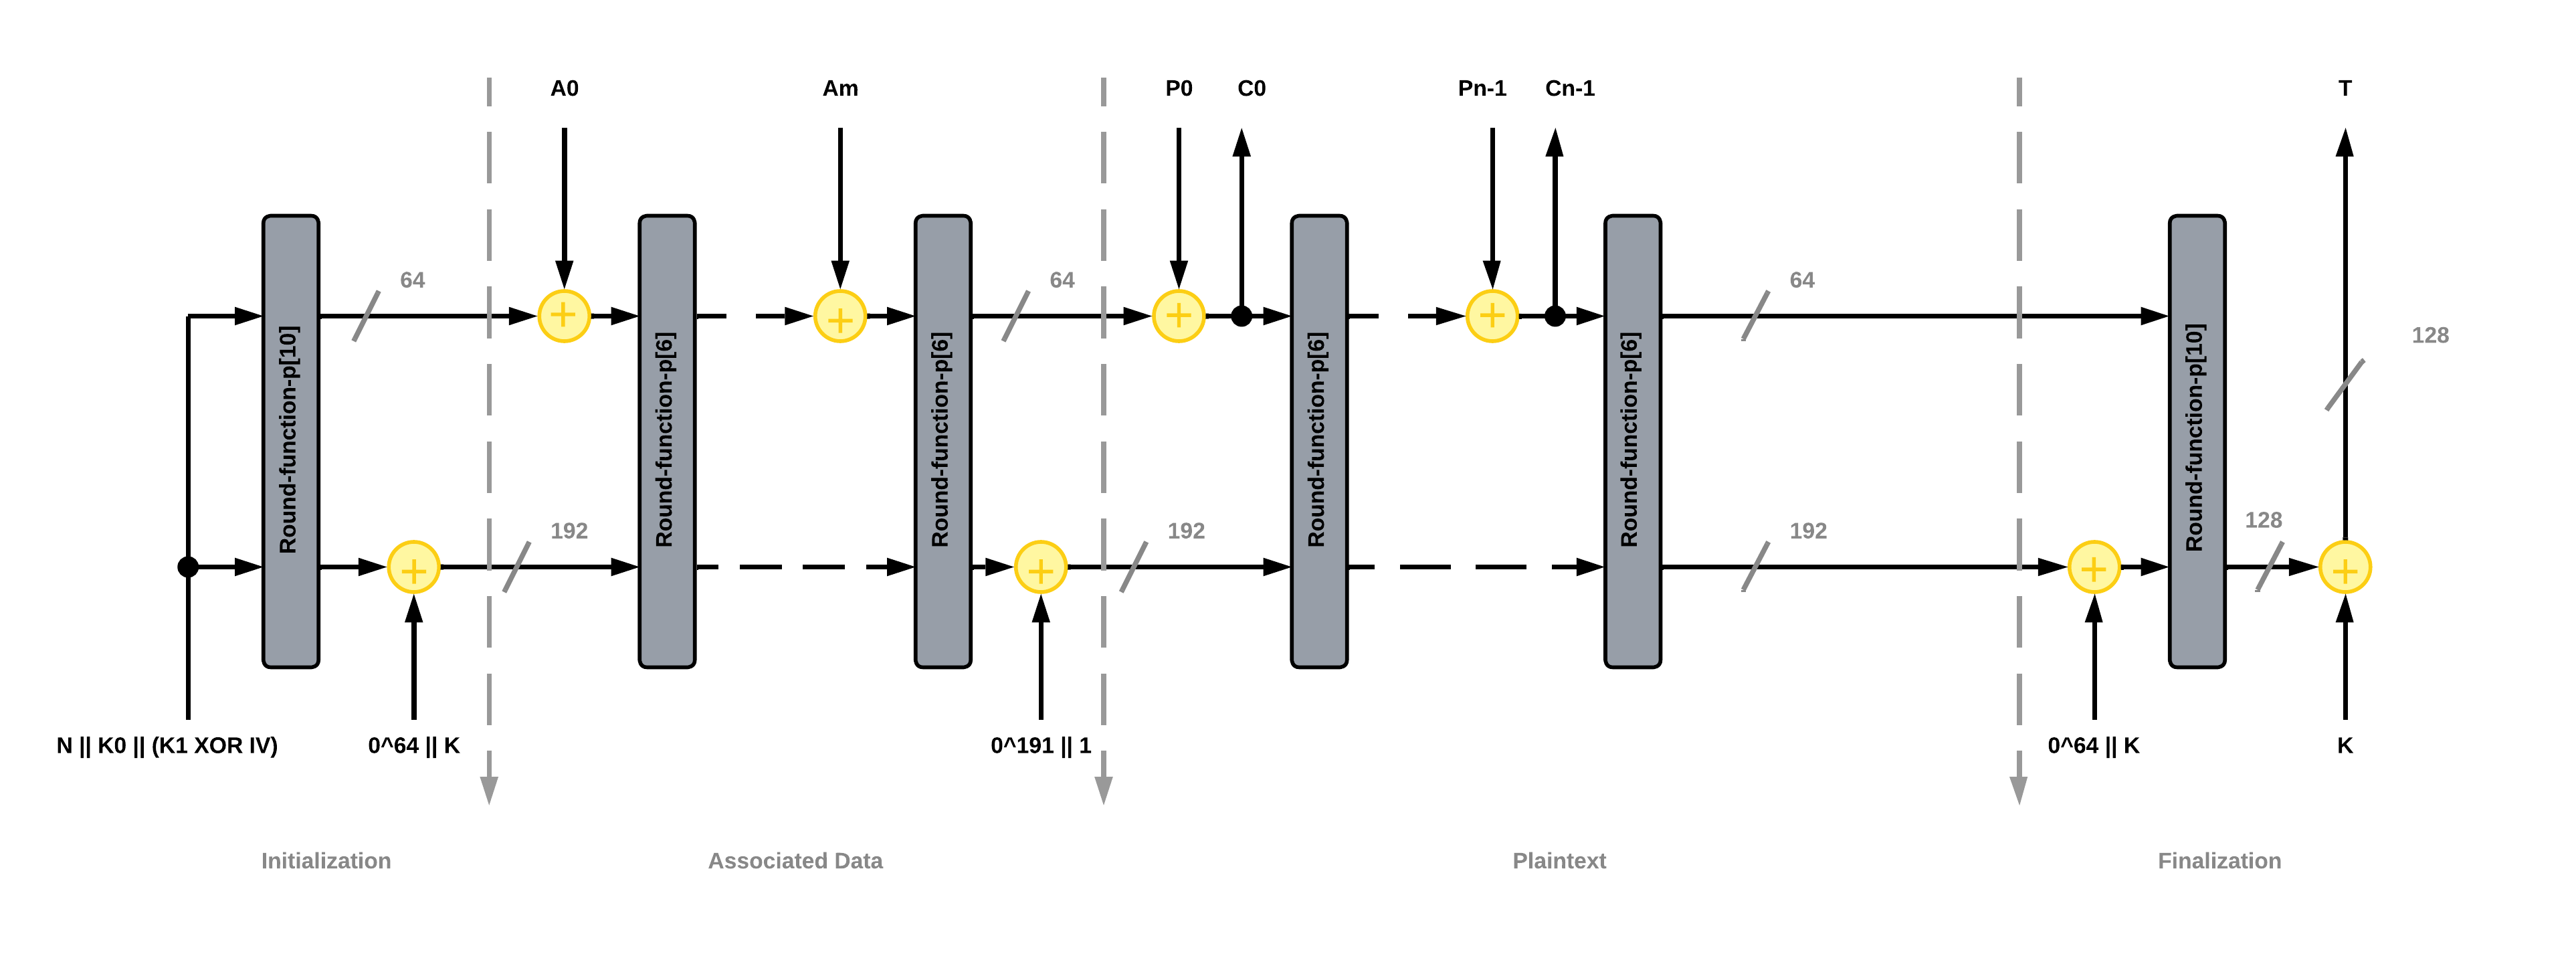
\includegraphics[width=\textwidth]{images/sipcon-mode}
\caption{SipCon64's operating mode. The top line is the 64-bit rate $x_0$, where all data enters and leaves. The bottom line is the 192-bit capacity $x_1,x_2,x_3$, which keeps the system secure by never directly touching outside data. We use $p^{10}$ at the start and end, injecting the key both times. We use $p^{6}$ between data blocks. The extra bit added before the plaintext phase is the domain separator from \eqref{eq:dsep}.}
\label{fig:mode}
\end{figure*}

Fig.~\ref{fig:mode} outlines the four main phases.

\subsubsection{Padding}
\label{sec:padding}
Two of those phases end with a block that may be only partly filled, and both
close it the same way. Padding is not a separate step in the diagram: it
happens \emph{inside} the last absorption of the associated-data phase and
again inside the last absorption of the plaintext phase, and Fig.~\ref{fig:mode}
does not draw it.

Let $\ell$ be the number of message bits in that final block, $0 \le \ell < r$.
The block is absorbed into the low $\ell$ bits of the rate, the ciphertext is
taken from those same $\ell$ bits, and a single \texttt{1} bit followed by
zeros is then exclusive-ored into the $r-\ell$ bits above them:
\begin{equation}
S_r \leftarrow S_r \oplus (0^{\ell} \,\|\, 1 \,\|\, 0^{\,r-1-\ell}).
\label{eq:pad}
\end{equation}
In the implementation this is the single byte \texttt{0x01} placed at byte
offset $\ell/8$ of $x_0$, and it is applied \emph{after} the ciphertext has
been extracted, so the padding never reaches the output. Because it touches
only bits the message did not occupy, it marks unambiguously where the data
ended and prevents two messages of different length from leaving the state in
the same condition.

Fig.~\ref{fig:mode} sets out the block structure of each phase; the padding
rule that brings every block up to $r$ bits is carried by \eqref{eq:pad} rather
than drawn. Under that rule a closing fragment of $\ell$ bits becomes the full
block $M \,\|\, 1 \,\|\, 0^{\,r-1-\ell}$, so the permutation always receives
$r$ bits whatever the message length. SipCon64 follows Ascon \cite{caesar} here
unchanged.

\subsubsection{Initialization}
We load the nonce and the key, mix the state, and then inject the key again:
\begin{align}
S &\leftarrow N_0 \,\|\, N_1 \,\|\, K_0 \,\|\, (K_1 \oplus \mathit{IV}),
\nonumber\\
S &\leftarrow p^{10}(S) \oplus (0^{128} \,\|\, K).
\label{eq:init}
\end{align}
Because SipCon64 only has four words, it does not have a spare word to hold the IV like Ascon does. Instead, it merges the IV directly into the key ($K_1$) while the nonce takes up $x_0,x_1$.

\subsubsection{Associated data}
We mix each 64-bit chunk of extra data into the rate and run 6 rounds:
\begin{equation}
S \leftarrow p^{6}\big((S_r \oplus A_i) \,\|\, S_c\big),
\qquad 1 \le i \le s,
\label{eq:ad}
\end{equation}
After all chunks are handled, we flip a single bit to separate this phase from the next:
\begin{equation}
S \leftarrow S \oplus (0^{255} \,\|\, 1).
\label{eq:dsep}
\end{equation}
Just like Ascon, we flip this bit \emph{even if there was no extra data provided}. This prevents the system from confusing an empty data phase with the start of the message. Fig.~\ref{fig:mode} shows this bit landing in the capacity section ($0^{191}\Vert{}1$), which translates to the byte \texttt{0x80} at the top of $x_3$.

\subsubsection{Plaintext}
We combine each message block with the rate to create the ciphertext output:
\begin{equation}
C_i \leftarrow S_r \oplus P_i, \qquad
S \leftarrow
\begin{cases}
p^{6}(C_i \,\|\, S_c) & 1 \le i < t\\
C_i \,\|\, S_c & i = t,
\end{cases}
\label{eq:pt}
\end{equation}
We cut the final block to the exact size of the message and do not run a mixing step afterward.

\subsubsection{Finalization}
We inject the key, mix the state a final time, and extract the tag from the last two words:
\begin{align}
S &\leftarrow p^{10}\big(S \oplus (0^{128} \,\|\, K)\big),
\nonumber\\
T &\leftarrow \lfloor S \rfloor_{128} \oplus K.
\label{eq:final}
\end{align}
Ascon injects the key into different spots before and after this final mix. SipCon64 injects the key into the exact same spot both times (the last two words, $x_2$ and $x_3$) because that is where we pull the final tag from.

\subsection{Encryption and Decryption}

Algorithms~\ref{alg:enc} and~\ref{alg:dec} detail the entire process. They only differ in one specific way: encryption mixes the message into the rate, while decryption pulls the message out and then \emph{overwrites} the rate with the ciphertext. For the final partial block, it overwrites only the needed bits while leaving the leftover padding bits untouched.

\begin{algo}{$\mathrm{SipCon64\text{-}Enc}(K, N, A, P)$}\label{alg:enc}
\areq{128-bit key $K=K_0\|K_1$, 128-bit nonce $N=N_0\|N_1$, associated data $A$, plaintext $P$}
\aens{ciphertext $C$, 128-bit tag $T$}
\aphase{Initialization phase}
\aln $x_0 \leftarrow N_0$;\ \ $x_1 \leftarrow N_1$;\ \ $x_2 \leftarrow K_0$;\ \ $x_3 \leftarrow K_1 \oplus \mathit{IV}$
\aln $S \leftarrow p^{10}(S)$
\aln $x_2 \leftarrow x_2 \oplus K_0$;\ \ $x_3 \leftarrow x_3 \oplus K_1$
\aphase{Associated data phase}
\aln \kw{if} $|A| > 0$ \kw{then}
\aln[1] $A_1 \dots A_s \leftarrow 64$-bit blocks of $A\|1\|0^{*}$
\aln[1] \kw{for} $i = 1$ \kw{to} $s$ \kw{do}
\aln[2] $x_0 \leftarrow x_0 \oplus A_i$
\aln[2] $S \leftarrow p^{6}(S)$
\aln[1] \kw{end for}
\aln \kw{end if}
\aln $x_3 \leftarrow x_3 \oplus \mathit{DSEP}$ \cmt{also if $s=0$}
\aphase{Plaintext phase}
\aln $P_1 \dots P_t \leftarrow 64$-bit blocks of $P\|1\|0^{*}$
\aln \kw{for} $i = 1$ \kw{to} $t-1$ \kw{do}
\aln[1] $C_i \leftarrow x_0 \oplus P_i$
\aln[1] $x_0 \leftarrow C_i$
\aln[1] $S \leftarrow p^{6}(S)$
\aln \kw{end for}
\aln $C_t \leftarrow x_0 \oplus P_t$;\ \ $x_0 \leftarrow C_t$ \cmt{no trailing $p^{6}$}
\aln $\tilde{C}_t \leftarrow \lfloor C_t \rfloor_{|P| \bmod r}$
\aphase{Finalization phase}
\aln $x_2 \leftarrow x_2 \oplus K_0$;\ \ $x_3 \leftarrow x_3 \oplus K_1$
\aln $S \leftarrow p^{10}(S)$
\aln $T \leftarrow (x_2 \oplus K_0) \,\|\, (x_3 \oplus K_1)$
\aunn[1] \kw{return} $C_1\|\dots\|C_{t-1}\|\tilde{C}_t$, $T$
\end{algo}

\begin{algo}{$\mathrm{SipCon64\text{-}Dec}(K, N, A, C, T)$}\label{alg:dec}
\areq{128-bit key $K=K_0\|K_1$, 128-bit nonce $N=N_0\|N_1$, associated data $A$, ciphertext $C$, tag $T$}
\aens{plaintext $P$, or $\bot$ on authentication failure}
\aphase{Initialization phase}
\aln $x_0 \leftarrow N_0$;\ \ $x_1 \leftarrow N_1$;\ \ $x_2 \leftarrow K_0$;\ \ $x_3 \leftarrow K_1 \oplus \mathit{IV}$
\aln $S \leftarrow p^{10}(S)$
\aln $x_2 \leftarrow x_2 \oplus K_0$;\ \ $x_3 \leftarrow x_3 \oplus K_1$
\aphase{Associated data phase}
\aln \kw{if} $|A| > 0$ \kw{then}
\aln[1] $A_1 \dots A_s \leftarrow 64$-bit blocks of $A\|1\|0^{*}$
\aln[1] \kw{for} $i = 1$ \kw{to} $s$ \kw{do}
\aln[2] $x_0 \leftarrow x_0 \oplus A_i$
\aln[2] $S \leftarrow p^{6}(S)$
\aln[1] \kw{end for}
\aln \kw{end if}
\aln $x_3 \leftarrow x_3 \oplus \mathit{DSEP}$ \cmt{also if $s=0$}
\aphase{Ciphertext phase}
\aln $C_1 \dots C_{t-1}\tilde{C}_t \leftarrow 64$-bit blocks of $C$, $0 \le |\tilde{C}_t| < r$
\aln \kw{for} $i = 1$ \kw{to} $t-1$ \kw{do}
\aln[1] $P_i \leftarrow x_0 \oplus C_i$
\aln[1] $x_0 \leftarrow C_i$ \cmt{rate replaced, not XORed}
\aln[1] $S \leftarrow p^{6}(S)$
\aln \kw{end for}
\aln $\ell \leftarrow |\tilde{C}_t|$
\aln $\tilde{P}_t \leftarrow \lfloor x_0 \rfloor_{\ell} \oplus \tilde{C}_t$
\aln $x_0 \leftarrow x_0 \oplus (\tilde{P}_t\|1\|0^{r-1-\ell})$ \cmt{no trailing $p^{6}$}
\aphase{Finalization phase}
\aln $x_2 \leftarrow x_2 \oplus K_0$;\ \ $x_3 \leftarrow x_3 \oplus K_1$
\aln $S \leftarrow p^{10}(S)$
\aln $T^{*} \leftarrow (x_2 \oplus K_0) \,\|\, (x_3 \oplus K_1)$
\aln \kw{if} $T^{*} \ne T$ \kw{then return} $\bot$ \cmt{constant time}
\aunn[1] \kw{return} $P_1\|\dots\|P_{t-1}\|\tilde{P}_t$
\end{algo}

\subsection{Round-per-Cycle Hardware Realization}

The hardware version runs one full round every clock cycle. It uses a single 256-bit memory register, one block of math logic, and a basic controller. Since every phase uses the exact same mixing logic, the controller simply keeps track of the current phase. A 4-bit counter picks the round constant, starting at 2 for 10 rounds and 6 for 6 rounds, counting up to 11 both times.

Data moves in and out through 64-bit ports. A simple mask handles padding instantly during the exact same step the data is mixed. Encryption and decryption share almost all the same wiring; the only difference is whether the system mixes the incoming block or overwrites the rate entirely.

Processing $n_A$ data blocks and $n_M \ge 1$ message blocks takes this many cycles:
\begin{equation}
10 + 6,n_A + 6,(n_M - 1) + 10 \ \text{cycles},
\label{eq:cycles}
\end{equation}
compared to Ascon-AEAD128's $12 + 8n_A + 8(n_M-1) + 12$ over larger blocks. Because the system runs one round per cycle, the speed is directly limited by the two addition steps stacked on top of each other (Fig.~\ref{fig:round}). We cannot remove this delay without splitting the round into multiple cycles or using less accurate math, neither of which we do here.



\section{Implementation and Evaluation Flow}
\label{sec:impl}

\section{Results}
\label{sec:results}

\section{Discussion}
\label{sec:discussion}

\section{Conclusion}
\label{sec:conclusion}

%%% ------------------------------------------------------------------
%%% Bibliography. IEEEtran.bst is vendored alongside this file.
%%% Build: pdflatex main && bibtex main && pdflatex main && pdflatex main
%%% ------------------------------------------------------------------

\bibliographystyle{IEEEtran}
\bibliography{refs}

%%% ------------------------------------------------------------------
%%% Author photographs and biographies are not required at initial
%%% submission but will be requested at revision. Uncomment and fill in;
%%% the space they occupy must fit inside the 14-page hard limit.
%%% ------------------------------------------------------------------
%
% \begin{IEEEbiography}[{\includegraphics[width=1in,height=1.25in,clip,keepaspectratio]{photo.jpg}}]{Kaushal Shinde}
% Biography text here.
% \end{IEEEbiography}

\end{document}
